%Übersicht ist in getrennter Datei audio-uebersicht.
\hyphenation{
Au-dio-stream
Bit-ra-te
FFmpeg
WAVE
}
\paragraph{Vertiefung} Die eigentlichen Audiodaten werden in einem eigenen Format gespeichert, dem sogenannten Codec, welcher wiederum in einem Containerformat eingebettet wird. Nähere Erläuterungen dazu sind in dem Kapitel Video in den Unterabschnitten Containerformat ab Seite \pageref{video-container} sowie Codec und Kompression ab Seite \pageref{video-codec} zu finden.

Die Qualität einer Audiodatei ist zu einem großen Teil von der Abtastrate und Abtasttiefe abhängig. Die Anzahl der Tonkanäle und deren Anordnung werden mittels der Angabe des Tonsystems beschrieben, welche notwendig ist, um die Datei korrekt abzuspielen.

Die Datenmenge von Audiodaten ist nicht nur von der Abtastrate und der Abtasttiefe, sondern auch von der Bitrate abhängig. In dem Kapitel Video wird dieser Begriff in dem Unterabschnitt Datenrate ab Seite \pageref{video-datenrate} erläutert.

\subparagraph{Abtastrate und Abtasttiefe}
Mit analoger Technik kann Ton so aufgenommen werden, wie er physikalisch auftritt, nämlich als durchgängige Schallwelle. Um dieses Signal zu digitalisieren muss es in bestimmten Zeitintervallen gemessen und gespeichert werden. Die Zeitintervalle, also die Häufigkeit, in der das Signal gemessen wird, wird als Abtastrate bezeichnet. Je kleiner das Zeitintervall, desto größer die Abtastrate und desto mehr entspricht das digitale Signal dem analogen Signal. Die Abtastrate wird meist in Kilohertz (kHz) angegeben.

Wie genau der gemessene und gespeicherte Wert dann dem ursprünglichen Signal entspricht, hängt von der Messgenauigkeit ab. Diese Messgenauigkeit wird durch die Anzahl der Bits bestimmt und wird als Abtasttiefe bezeichnet. Sie ist vergleichbar mit der Farbtiefe, die in dem Kapitel über Rastergrafiken ab Seite \pageref{RG_Farbtiefe} beschrieben wird. Je größer die Abtasttiefe, desto feiner kann das Signal gemessen werden und die ursprüngliche Tonqualität reproduziert werden.

Eine höhere Abtastrate und eine größere Abtasttiefe führen zu einer originalgetreueren digitalen Repräsentation des Signals.

Der gemessene Wert des Signals kann zwischen zwei Werten der durch die Messgenauigkeit vorgegebenen Messskala liegen, weshalb dieser auf den nächstliegenden Wert gerundet werden muss. Dieser Vorgang wird als Quantisierung bezeichnet.

\begin{figure}[!htp]
  \begin{center}
    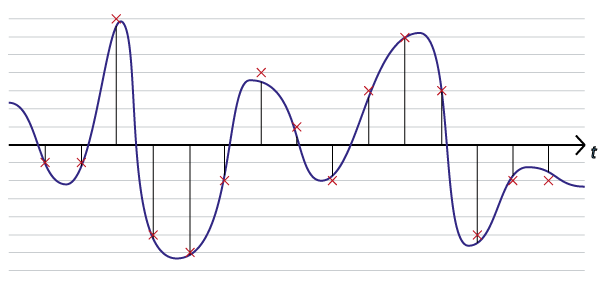
\includegraphics[width=0.9\textwidth]{bilder/audio_abtastrateAbtasttiefe}
  \end{center}
	\caption{Die Abtastung und Quantisierung eines Schallsignals. Das Schallsignal (blau) wird in einem vorgegebenen Intervall (senkrechte Linien) gemessen. Der gemessene Wert wird auf den nächstgelegenen Wert der durch die Abtasttiefe vorgegebenen Skala (horizontale Linien) quantisiert (Kreuze), weshalb die digitale Repräsentation des Signals leicht abweicht.}
\end{figure}

Puls-Code-Modulation (PCM) bezeichnet das Abtasten eines Signals in einer vorgegebenen Abtastrate und die anschließende Quantisierung des gemessenen Wertes. Die lineare Puls-Code-Modulation verwendet dabei einen immer gleich groß bleibenden Wertebereich, also immer die gleiche Messskala für die abgetasteten Werte.


\subparagraph{Tonkanäle und Tonsysteme}
Bei der Wiedergabe von Audiodateien, beispielsweise über Kopfhörer, besteht die Möglichkeit Töne nur auf einem der beiden Hörer auszugeben, um einen räumlichen Schalleindruck zu erzeugen. Dafür werden technisch die in der Audiodatei gespeicherten Tonkanäle (Tonspuren) verwendet und an die unterschiedlichen Ausgabegeräte geleitet, wie etwa an den linken und den rechten Kopfhörer.

In einer Audiodatei können eine, zwei oder noch mehr Tonspuren enthalten sein. Dabei kann die intendierte Anordnung der Lautsprecher je nach Anzahl der Kanäle variieren. Bei einer Tonspur wird davon ausgegangen, dass sich das Ausgabegerät vor dem Hörer befindet und bei zwei Tonspuren von zwei Ausgabegeräten links und rechts vom Hörer. Ab drei Kanälen sind mehr als zwei Anordnungen möglich, weshalb die Benennung des Tonsystems oder eine Angabe zur Anordnung notwendig wird. 

%XXX Grafik? Mit den Symbolen, um zu zeigen, dass die Anordung variieren kann


\paragraph{Praxis}
Dieser Abschnitt vereint Hinweise zum Umgang mit Audiodaten. Es gibt Erläuterungen mit Literatur- und Programmhinweisen über die Ansicht und Extraktion von Metadaten, die Aufnahme, die Wiedergabe und die Transcodierung von Audiodateien. Für die Aufnahme und Digitalisierung von Ton werden Mindestanforderungen spezifiziert und Hinweise auf vertiefende Informationen gegeben.


\subparagraph{Metadaten}Die technischen Metadaten sind in der Regel in dem Header der Datei gespeichert und können von verschiedenen Programmen ausgelesen werden. Ein Programm, das mit vielen Formaten umgehen kann und auch den Export von Metadaten in eine gesonderte Datei erlaubt ist MediaInfo.

Zu den Exportformaten gehören PBCore und EBUCore. Es handelt sich dabei um Metadatenschemata, die speziell für Film und Ton von Public Broadcasting in den USA, beziehungsweise von der European Broadcasting Union (EBU) entwickelt wurden. Die Moving Pictures Experts Group (MPEG) hat MPEG-7 für die Dokumentation von Multimediadateien entwickelt, der insbesondere zur Erweiterung der anderen MPEG-Standards gedacht ist.

Für das Editieren von Metadaten im BWF-Format gibt es das Programm BWF MetaEdit.

\begin{flushleft}
	MediaInfo: \urllist{https://mediaarea.net/MediaInfo}
	PBCore: \urllist{http://pbcore.org/}
	EBUCore: \urllist{https://tech.ebu.ch/MetadataEbuCore}
	MPEG-7: \urllist{http://mpeg.chiariglione.org/standards/mpeg-7}
	BWF MetaEdit: \urllist{https://sourceforge.net/projects/bwfmetaedit/}
\end{flushleft}


\subparagraph{Aufnahme und Bearbeitung}
Für die Aufnahme und Bearbeitung von Audiodaten kann das kostenlose Programm Audacity verwendet werden. Audacity gibt es für alle gängigen Betriebssysteme.

Bei der Aufnahme sollte auf eine angemessene Aufnahmequalität geachtet werden. In der Handreichung \href{http://www.dfg.de/download/pdf/foerderung/grundlagen_dfg_foerderung/informationen_fachwissenschaften/geisteswissenschaften/standards_sprachkorpora.pdf}{\emph{Empfehlungen zu datentechnischen Standards und Tools bei der Erhebung von Sprachkorpora}} der DFG werden eine Abtastrate von 22 kHz und eine Abtasttiefe von 16 bit als Mindestanforderungen spezifiziert. Jedoch ist eine höhere Abtastrate von 48 kHz empfehlenswert, da diese eher der Grenzfrequenz des menschlichen Gehörs entspricht, besser wären sogar 96 kHz. Die Abtastung sollte linear erfolgen.

Welche Abtastrate sich für die gewünschte Aufnahme am besten eignet, kann mittels der Nyquist-Frequenz ermittelt werden. Die Nyquist-Frequenz besagt, dass das originale Signal exakt reproduziert werden kann, wenn die Abtastrate doppelt so hoch wie die höchste Signalfrequenz ist.

\begin{figure}[!htp]
  \begin{center}
    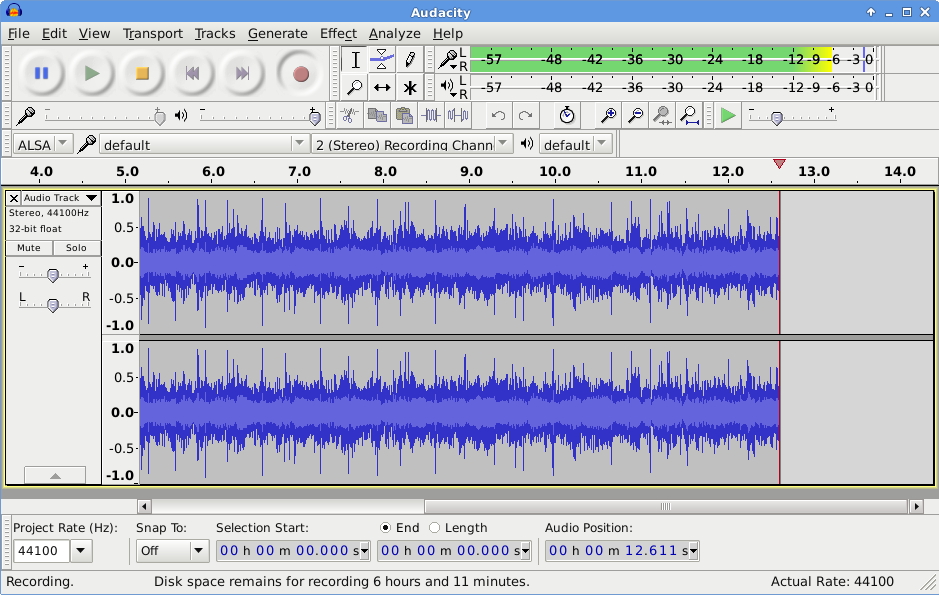
\includegraphics[width=0.9\textwidth]{bilder/audio_audacity}
  \end{center}
	\caption{Audacity (audacity.org)}
\end{figure}

\begin{flushleft}
	Audacity: \urllist{http://www.audacityteam.org/}
	Handreichung der DFG: \urllist{http://www.dfg.de/download/pdf/foerderung/grundlagen_dfg_foerderung/informationen_fachwissenschaften/geisteswissenschaften/standards_sprachkorpora.pdf}
\end{flushleft}


\subparagraph{Wiedergabeprogramme} Jedes Betriebssystem hat meist schon ein Programm für die Wiedergabe von Audiodateien vorinstalliert. Jedoch können diese Programme nur mit einer begrenzten Auswahl von Containerformaten und Codecs umgehen. Codecs können nachträglich installiert werden, wobei aber auf Kompatibilität mit dem Wiedergabeprogramm geachtet werden muss.

Ein Programm, das mit allen hier vorgestellten Formaten und Codecs umgehen kann, ist der VLC media player. Unter der unscheinbaren Oberfläche verbirgt sich eine Vielzahl an Funktionalitäten und das Programm gibt es für alle gängigen Betriebssysteme.

\begin{flushleft}
	VLC media player von VideoLAN: \urllist{http://www.videolan.org/vlc/index.html}
\end{flushleft}


\subparagraph{Transcodierung} Für die Transcodierung, also die Konvertierung von einem Codec in einen weiteren gibt es einige frei verfügbare Programme, wie beispielsweise der bereits genannte VLC media player, der eine leicht verständliche grafische Oberfläche anbietet. Für fortgeschrittene Anwender ist das ebenfalls frei verfügbare FFmpeg zu empfehlen, das komplexere und detailliertere Transcodierungsoptionen erlaubt und auch von der Kommandozeile aus gesteuert werden kann. 

\begin{flushleft}
	VLC media player von VideoLAN: \urllist{http://www.videolan.org/vlc/index.html}
	FFmpeg: \urllist{https://www.ffmpeg.org/}
\end{flushleft}


\subparagraph{Digitalisierung}
Für die Digitalisierung von analogem Audiomaterial gibt es von der IASA konkrete Vorgaben, die eine minimale Abtastrate von 48 kHz und eine minimale Abtasttiefe von 24 Bits empfehlen, um eine möglichst hohe Qualität des Digitalisats zu gewährleisten. Als Formate werden WAVE oder BWF mit linearem PCM vorgegeben. Ausführliche Hinweise sind in den \href{http://www.iasa-web.org/tc04/audio-preservation}{Guidelines on the Production and Preservation of Digital Audio Objects (IASA-TC 04)} der IASA zu finden. 

Es sollte darauf geachtet werden, dass das originale analoge Material weiterhin erhalten bleibt und die Konsultierung eines darauf spezialisierten Archivs oder Dienstleisters ist ratsam.

\paragraph{Quellen}
\begin{flushleft}
Archaeology Data Service, Digital Audio: A Guide to Good Practice \urllist{http://guides.archaeologydataservice.ac.uk/g2gp/Audio_Toc}
Hicks, Tony, Should We Be Using ISO 12083?, The Journal of Electronic Publishing 3, 1998, 4 \urllist{http://quod.lib.umich.edu/j/jep/3336451.0003.407?view=text;rgn=main}

W. Bergmeyer, Audio, In: H. Neuroth -- A. Oßwald -- R. Scheffel -- S. Strathmann -- K. Huth (Hrsg.) nestor Handbuch. Eine kleine Enzyklopädie der digitalen Langzeitarchiverung. Version 2.3 (2010) Kap. 17.6 \urllist{http://www.nestor.sub.uni-goettingen.de/handbuch}

V. Ernst -- J. Kepier -- J. Renz -- A. Romeyke -- T. Bähr, Leitfaden für die digitale Langzeitarchivierung audiovisueller Medien (2016) \urllist{http://nbn-resolving.de/urn:nbn:de:0008-2016102107}

FADGI (Hrsg.), Guidelines: Embedded Metadata in Broadcast WAVE Files \urllist{http://www.digitizationguidelines.gov/guidelines/digitize-embedding.html}

IASA (Hrsg.), Guidelines on the Production and Preservation of Digital Audio Objects (IASA-TC 04) \urllist{http://www.iasa-web.org/tc04/audio-preservation}

JISC (Hrsg.), Infokit: Digital file formats. Audio \urllist{http://www.jiscdigitalmedia.ac.uk/infokit/file_formats/digitisation-audio}

JISC (Hrsg.), Infokit: Digital file formats. Digital audio formats and compression \urllist{http://www.jiscdigitalmedia.ac.uk/infokit/file_formats/digital-audio-formats-and-compression}

Koordinationsstelle für die dauerhafte Archivierung elektronischer Unterlagen (Hrsg.) Katalog archivischer Dateiformate: Audiodaten \urllist{http://kost-ceco.ch/wiki/whelp/KaD/pages/Audio.html}

R. Kromer, On Audio-Visual File Formats (Notizen zur Präsentation 2015) \urllist{http://reto.ch/training/2015/20150424/audio.html}

Memoriav (Hrsg.), Memoriav Empfehlungen Ton. Die Erhaltung von Tondokumenten (2014) \urllist{http://memoriav.ch/wp-content/uploads/2015/02/Empfehlungen_Ton_de.pdf}

Y. Trivedi, HTG Explains: What Are the Differences Between All Those Audio Formats? (2011) \urllist{http://www.howtogeek.com/howto/40465/htg-explains-what-are-the-differences-between-all-those-audio-formats/}

Wikipedia Mehrkanal-Tonsystem (deutsch 05. 2016) \urllist{https://de.wikipedia.org/wiki/Mehrkanal-Tonsystem}

\quelltyp{Formatspezifikationen}
FLAC: \urllist{https://xiph.org/flac/format.html}
WAVE: McGill University \urllist{http://www-mmsp.ece.mcgill.ca/documents/audioformats/wave/wave.html}
WAVE mit LCPM: Library of Congress \urllist{http://www.digitalpreservation.gov/formats/fdd/fdd000002.shtml}
WAVE als Teil von RIFF: \urllist{http://www.tactilemedia.com/info/MCI_Control_Info.html}
BWF: \urllist{http://tech.ebu.ch/docs/tech/tech3285.pdf}
MBWF/RF64: \urllist{http://tech.ebu.ch/docs/tech/tech3306-2009.pdf}
Matroska: \urllist{https://www.matroska.org/}
Matroska: Library of Congress \urllist{http://www.digitalpreservation.gov/formats/fdd/fdd000342.shtml}
Matroska: IETF CELLAR Charter \urllist{https://datatracker.ietf.org/doc/charter-ietf-cellar/}
MP3 (MPEG-1): \urllist{http://mpeg.chiariglione.org/standards/mpeg-1}
MPEG-1: Library of Congress \urllist{http://www.digitalpreservation.gov/formats/fdd/fdd000035.shtml}
AAC (MPEG-4): \urllist{http://mpeg.chiariglione.org/standards/mpeg-4}
MP4 mit AAC: Library of Congress \urllist{http://www.digitalpreservation.gov/formats/fdd/fdd000234.shtml}

\quelltyp{Tools und Programme}
MediaInfo: \urllist{https://mediaarea.net/MediaInfo}
PBCore: \urllist{http://pbcore.org/}
EBUCore: \urllist{https://tech.ebu.ch/MetadataEbuCore}
MPEG-7: \urllist{http://mpeg.chiariglione.org/standards/mpeg-7}
BWF MetaEdit: \urllist{https://sourceforge.net/projects/bwfmetaedit/}
Audacity: \urllist{http://www.audacityteam.org/}
VLC media player von VideoLAN: \urllist{http://www.videolan.org/vlc/index.html}
FFmpeg: \urllist{https://www.ffmpeg.org/}
\end{flushleft}